\chapter{Tidsplan}
Fra starten af lagde vi en plan over delmålene vi havde. Denne plan fremgår af figur \ref{fig:tidsplan1}. Som det kan ses var planen at starte med basic-delmålene og derfra bevæge os ud mod de mere avancerede som liv, hastighed, score, internt koordinatsystem, sværhedsgrader osv. Efterfølgende ville vi implementere et DEXXA Steering Wheel til sjovere controller-styring af spillet.\\
Efter dette ville vi begynde på hvad man kan kalde en finpudsning af spillet. Dvs. ordentlig start menu og beskeder hvis spillet vindes eller tabes. \\

Efterfølgende ville vi lave power-up's og power-down's til spillet. Vi fandt lynhurtigt masse potentielle af disse, såsom at strikeren kunne blive bredere/smallere, bolden kunne klistre til strikeren, bolden kunne skydes direkte igennem brikkerne uden at blive reflekteret, størrelsen og hastigheden af bolden kunne ændres osv. Vi fandt hurtigt ud af det i det achievements-delmål nok ville blive meget tidskrævende og derfor satte vi det som det tredje sidste punkt i planen, lige før fintuning og rapportskrivning.\\ \\


\begin{figure}[h!]
\centering
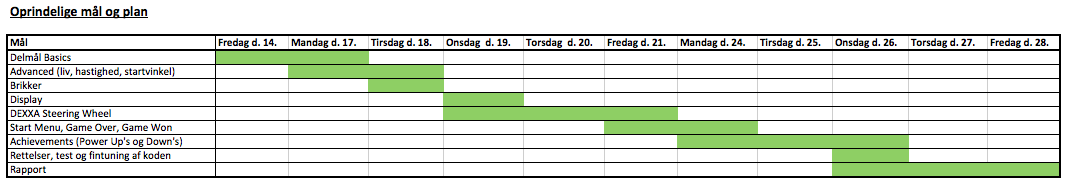
\includegraphics[scale=0.4]{figs/Tidsplan1.png}
\caption{Tidsplan over de forskellige delmål og hvornår de skulle være færdige}
\label{fig:tidsplan1}
\end{figure}